\label{chap:communication}
\label{sec:communication}

This chapter describes the communication interface between the GUI and the User Space, which is based on Remote Procedure Calls.

\section{Remote Procedure Calls}
\label{sec:rpc:rpc}

GUI communicates with User Space via the Google Web Toolkit RemoteService implementation.

\subsection{RPC in general}
A \emph{remote procedure call} is a method providing interaction between the client (the GUI) and the server (the User Space).

From the start, it was obvious to us that we want to use a well-established method to implement the Remote Procedure Calls. GWT provides a ready-to-use Remote Service implementation, where the programmer only has to define the set of RPCs as an interface, implement the interface on the server side, and invoke an RPC on the client side by implementing the GWT {\tt AsyncCallback} interface.
Everything else is handled automatically and transparently by GWT.

The type of an RPC parameter or its return value can be any GWT-compilable type. Because this type must be known both to the server and to the client, we use only primitive types and shared classes. Each class sendable through the GWT RPC mechanism must implement the GWT {\tt IsSerializable} interface (which is only a marker, i.e.\ it does not have any abstract methods) and a parameter-less constructor; this also holds for the checked exceptions, which are technically only a special type of return value.

\subsection{Our implementation}
The shared class {\tt FilmTitService} \emph{defines} the FilmTitService interface, an API for communication, by specifying the RPCs as methods with a name, a set of parameters, a return type and checked exceptions. The User Space class {\tt FilmTitBackendServer} must \emph{implement} each of the defined RPCs. The interface provides \emph{asynchronous} RPC methods -- the responses are processed by \emph{callbacks}. A class in {\tt cz.filmtit.client.callables} may \emph{invoke} the RPC, passing the required parameters to the GWT RPC mechanism which ensures their delivery to the server and the execution of the implementation method.

The callable class must implement an asynchronous callback by implementing the methods {\tt onSuccess()} and {\tt onFailure()}, which are called by the GWT RPC mechanism when the RPC \emph{returns}, i.e.\ returns a value or fails with an exception and the result is received by the GUI. Failure is defined as the RPC server implementation throwing an exception, which is passed as a parameter to {\tt onFailure()}. Otherwise, the returned value is passed to {\tt onSuccess()}.
In case of common points of failure that do not qualify as an exceptional state, such as user registration attempt with an already existing username, the common failure is typically signaled by the return value instead (typically a null or a false).

The RPC is always invoked from the client, because JavaScript security policies do not allow to handle incoming calls.
Therefore, in case the User Space needs to actively contact the GUI without the GUI having sent a request before,
this has to be implemented in the GUI by polling.

Most of the RPCs can only be invoked by a logged-in user. Such RPCs always have the sessionID as their first parameter to authenticate the user and can throw an {\tt InvalidSessionIdException}.
A {\tt sessionID} is a unique identifier of a logged in user, valid for 1 hour (or 1 month if the user decided to be ``permanently logged in''), managed by the User Space.

The parameters, return values and exceptions thrown must be GWT-serializable, and their types must be supported both by GUI and User Space. Therefore, we either use types supported both by GWT and Java (such as int, String or List) or the Shared classes (see Section~\ref{sec:shared_classes}).

\subsection{Some issues}

Because of JavaScript and browser limitations, the RPC mechanism of GWT only allows asynchronous calls from client to server. This suited our needs often, but we had to go around these limits in some situations. Quite often, we need the RPC to be synchronous and blocking, e.g.\ in logging in or changing user settings. In such situations, the page or dialog is ``deactivated'' on invoking the RPC (all active components are disabled -- e.g.\ the text boxes are read-only, the buttons do not respond to clicks), a reference to the page or dialog is passed to the class invoking the RPC, and when the RPC returns, the page or dialog is ``reactivated'', either with a success message or an error message, depending on the result of the RPC.

In one case, we would need an opposite direction RPC, i.e.\ the server to invoke the RPC on the client. This is when authenticating the user through OpenID, where we have to perform the authentication in a new window -- the new window then receives the result of the authentication, but it cannot be easily passed directly into the opener window. Here, we decided to use active polling -- the opener window regularly invokes the {\tt GetSessionID} RPC, which returns null if the authentication process has{ not yet finished, this being a signal for the GUI to continue polling. To link together the opener window and the authentication window, a unique {\tt authID}, generated by the User Space, is used.

\subsubsection{Failed RPC Requests Handling}

We decided that our general error handling strategy should be to try to solve all problems without user interaction, and to inform the user only about user-generated errors (such as incorrect SRT file format or session timeout) or critical errors (such as permanent loss of connection to server).

The first thing was to turn the calls into objects, so that they store their parameters and can be called again on failure. We also created a generic superclass for them, Callable, filled with the necessary boilerplate code and methods performing the default actions, to be overridden if necessary.

We identified the response that we usually get in case of network problems (it is a {\tt StatusCodeException} with the status code 0). The problems can be temporary or permanent; in case of temporary problems, the default response of showing an error message was found to be highly inappropriate, as it would suffice only to resend the call. Therefore, we introduced retrying the call for three more times in such a case with short delays, before showing an error message to the user.

The retrial of calls has proven to be an efficient way to deal with problems, so we decided to extend it to all types of failures. However, in case of non-network errors, we soon found that retrying the calls does not make sense in some situations; so we decided to keep the retrial as a default action which can be overridden in the extending classes.

We also added a timeout for each request after which the request is regarded as lost and is retried. Such a situation is not at all typical, but we need to expect  it to prevent the user from ``starvation'' (the user can always escape from any state by refreshing the page in the browser, but this can lead to an uncontrolled local data loss or even to objects being left in an inconsistent state -- such as a document without content).



\section{Manipulating Documents}
\label{sec:rpc:doc}

A document is always identified by its {\tt documentID} (a long number generated by User Space on document creation), therefore most of the methods have the {\tt documentID} as one of their parameters.

A chunk in the document can always be identified by its {\tt ChunkIndex}, but for convenience in some cases the whole chunk is sent instead.
First, we introduce all the RPCs manipulating the documents. Then, we illustrate a typical sequence of RPCs invoked on document creation.

\subsection{Sending translation results -- discussion}
\label{sec:rpc:discussion_sending_results}

At first, the translation suggestions from the Translation Memory were requested and sent for each chunk individually. This had the theoretical advantage that the user received each of the translation suggestions as soon as possible. However, we found the overhead of the RPC calls to be unreasonable. Not only was the overall time necessary to load all the suggestions too long, but also a typical browser was unable to handle such a large number of requests and usually froze for long periods of time, often unfreezing only after all of the suggestions arrived.

A simple solution seemed to be sending all of the chunks for translation in one request. However, such a request can take several minutes to complete, and we still wanted to keep the nice property of the application of showing the suggestions as soon as possible at least for the first lines -- so that the user can start the translation immediately. Thus, we decided to send the request in batches, starting with a small size of the batch for the beginning of the file and gradually increasing the batch size.

The first way to do that was an exponential increase, where each batch contains twice as many chunks as the previous one, starting with a batch of size one. This proved to solve the aforementioned problem of browser freezing; however, another problem arose. As the batch sizes grew larger and larger, the later requests often took several tens of seconds or even minutes to complete. Meanwhile, the user would often navigate away from the Translation Workspace, rendering the translation suggestions, including the currently being processed ones, obsolete. This was of course detected in GUI and the suggestions were thrown away on arrival, but still it meant that the server was working in vain for some time, possibly resulting in an unnecessarily slower responsiveness to other users (and even to the very same user as well).

We introduced two further solutions. The first and simple one was limiting the size of the batch to 64 chunks (which typically take at most 5 seconds on the server side), so that the amount of useless work could not grow too large. The second solution was to stop the translation suggestions from being generated on the server, by issuing a {\tt StopTranslationResults} request. (This breaks the typical model of processing the queries, where once a query is sent, its processing is not influenced by queries that arrive later.)

The two major issues with the {\tt StopTranslationResults} request were:

\begin{itemize}
	\item to interrupt the suggestions generating which is already in process (which is done in parallel for the chunks in the batch, making this even harder).
	\item to identify what to stop and what to let continue.
\end{itemize}

The first idea was to mark the whole document as closed, and to check this when generating the suggestions. However, this would cause problems if the same document was immediately reopened by the user, and even larger problems if the user already had the document opened twice -- this can easily happen by mistake, the logical reaction of the user is then to close one of the Translation Workspaces, and then he would stop receiving suggestions even in the other opened Workspace. Thus, we then decided to create an identifier for each Translation Workspace instance and to bind the {\tt StopTranslationResults} request to this identifier. However, we soon found out that this would require additional overhead only to handle this probably not very common situation, so we dropped that idea as well.

Finally, we decided for a compromise solution between those two. The {\tt StopTranslationResults} request is now bound to individual chunks, which now have an added boolean field {\tt isActive}. This field is set to true when the {\tt GetTranslationResults} request arrives to the server, for each of the chunks on the request. The {\tt StopTranslationResults} request contains a list of the chunks which translations should be stopped. On arrival of that request, User Space simply sets the {\tt isActive} field to false -- because User Space and Core share the same memory and because only references to the chunks are passed around, this change is visible in core even though the chunks have already been sent for translation. The necessary overhead is minimal, and there is no "false alarm" in the typical case. The only unsolved case is the situation where the same batch of chunks are sent for translation at the same time from two different instances of Translation Workspace with the same document opened, and then one of these Workspaces is closed, causing the suggestions generation to stop even for the batch from the other Workspace. Although this situation is unlikely and non-critical (the suggestions would be missing only for this one batch, the later batches would be translated correctly), we still offer a general solution by repeating all request on failure (unless it is obvious that the failure will reoccur).

\subsection{Whole Document Operations}

\subsubsection{DocumentResponse createNewDocument(String sessionID, String documentTitle, String movieTitle, String language, String moviePath)}

Creates the document
(without source chunks, which have to be added by calling {\tt saveSourceChunks}).
Returns the {\tt documentID}, together with media source suggestions based on {\tt movieTitle}.
     	
\subsubsection{Void selectSource(String sessionID, long documentID, MediaSource selectedMediaSource)}
Sets the media source of the document. The media source represents the movie or series which the subtitles come from.

\subsubsection{List<Document> getListOfDocuments(String sessionID)}
Returns all documents owned by the user, ordered by date and time of last change.

\subsubsection{Document loadDocument(String sessionID, long documentID)}
Returns the document with the given documentID, with source chunks but without translation suggestions (these have to be explicitely requested by getTranslationResults).

\subsubsection{Void changeDocumentTitle(String sessionID, long documentID, String newTitle)}
Sets a different title for the document.

\subsubsection{List<MediaSource> changeMovieTitle(String sessionID, long documentID, String newMovieTitle)}
Returns media source suggestions based on {\tt newMovieTitle}.
The movie title is not changed yet:
this is only done on calling {\tt selectSource}.
     	
\subsubsection{Void deleteDocument(String sessionID, long documentID)}
Remove the given document from the list of user\'s documents.
(The data might not be discarded immediately
as the translations still might be used to enrich the translation memory)	 

\subsection{Source Subtitles Operations}

\subsubsection{Void saveSourceChunks(String sessionID, List<TimedChunk> chunks)}
Save the given source chunks as the contents of the given document
(which was already created by calling {\tt createNewDocument}).

\subsubsection{Void setChunkStartTime(String sessionID, ChunkIndex chunkIndex, long documentID, String newStartTime)}
Change the start time of the given chunk to the new value. The value must be in the SRT format, i.e. hh:mm:ss,ttt.

\subsubsection{Void setChunkEndTime(String sessionID, ChunkIndex chunkIndex, long documentID, String newEndTime)}
Change the end time of the given chunk to the new value. The value must be in the SRT format, i.e. hh:mm:ss,ttt.

\subsubsection{Void setChunkTimes(String sessionID, ChunkIndex chunkIndex, long documentID, String newStartTime, String newEndTime)}
Change the start time and end time of the given chunk to the values. The values must be in the SRT format, i.e. hh:mm:ss,ttt.

\subsubsection{TranslationResult changeText(String sessionID, TimedChunk chunk, String newDbForm)}
Change the source text of the chunk,
resulting in new translation suggestions
which are sent as the result.

\subsubsection{Void deleteChunk(String sessionID, ChunkIndex chunkIndex, long documentID)}
Remove the chunk from the document, together with its translation if it exists.

\subsection{Target Subtitles Operations}

\subsubsection{TranslationResult getTranslationResults(String sessionID, TimedChunk chunk)}
Get the list of possible translations of the given chunk.
The {\tt TranslationResult} instance contains zero or more translation suggestions, which come from the Translation Memory and/or the Machine Translation System.

\subsubsection{List<TranslationResult> getTranslationResults(String sessionID, List<TimedChunk> chunks)}
Get the list of lists of possible translations of the given chunks.
Each TranslationResult instance contains zero or more translation suggestions, which come from the Translation Memory and/or the Machine Translation System.

\subsubsection{Void stopTranslationResults(String sessionID, List<TimedChunk> chunks)}
Stop generating translation results for the given chunks
(to be called after getTranslationResults has been called
with the given chunks but the results are suddenly not needed anymore).

\subsubsection{Void setUserTranslation(String sessionID, ChunkIndex chunkIndex, long documentID, String userTranslation, long chosenTranslationPairID)}
Save the user translation of the given chunk (no matter whether it is user\'s own translation or a suggestion taken over or post-edited).
The ID of the {\tt TranslationPair} chosen for post-editing is also sent, providing feedback which then can be used to improve future suggestions.

\subsection{Document Creation}

The sequence diagram \ref{rpc:sd:document_creation} illustrates a typical sequence of RPCs invoked to create a document, including interaction with the Freebase service and the Core.

First, an empty document is created by the {\tt createNewDocument} RPC. The Freebase service is queried for suggestions on the actual movie or series matching the given {\tt movieTitle}, from which one is then selected by the {\tt selectSource} RPC -- this enables the Core to provide translation suggestions ranked according to the closeness of movie genres. Meanwhile, the {\tt saveSourceChunks} RPC is invoked to store the contents of the document once the subtitles file is parsed.

When both {\tt selectSource} and {\tt saveSourceChunks} have returned, the {\tt getTranslationResults} RPC starts to be iteratively invoked to obtain translation suggestions, generated by the Core, until the whole document gets translation suggestions.

\begin{figure}[h]
\begin{center}
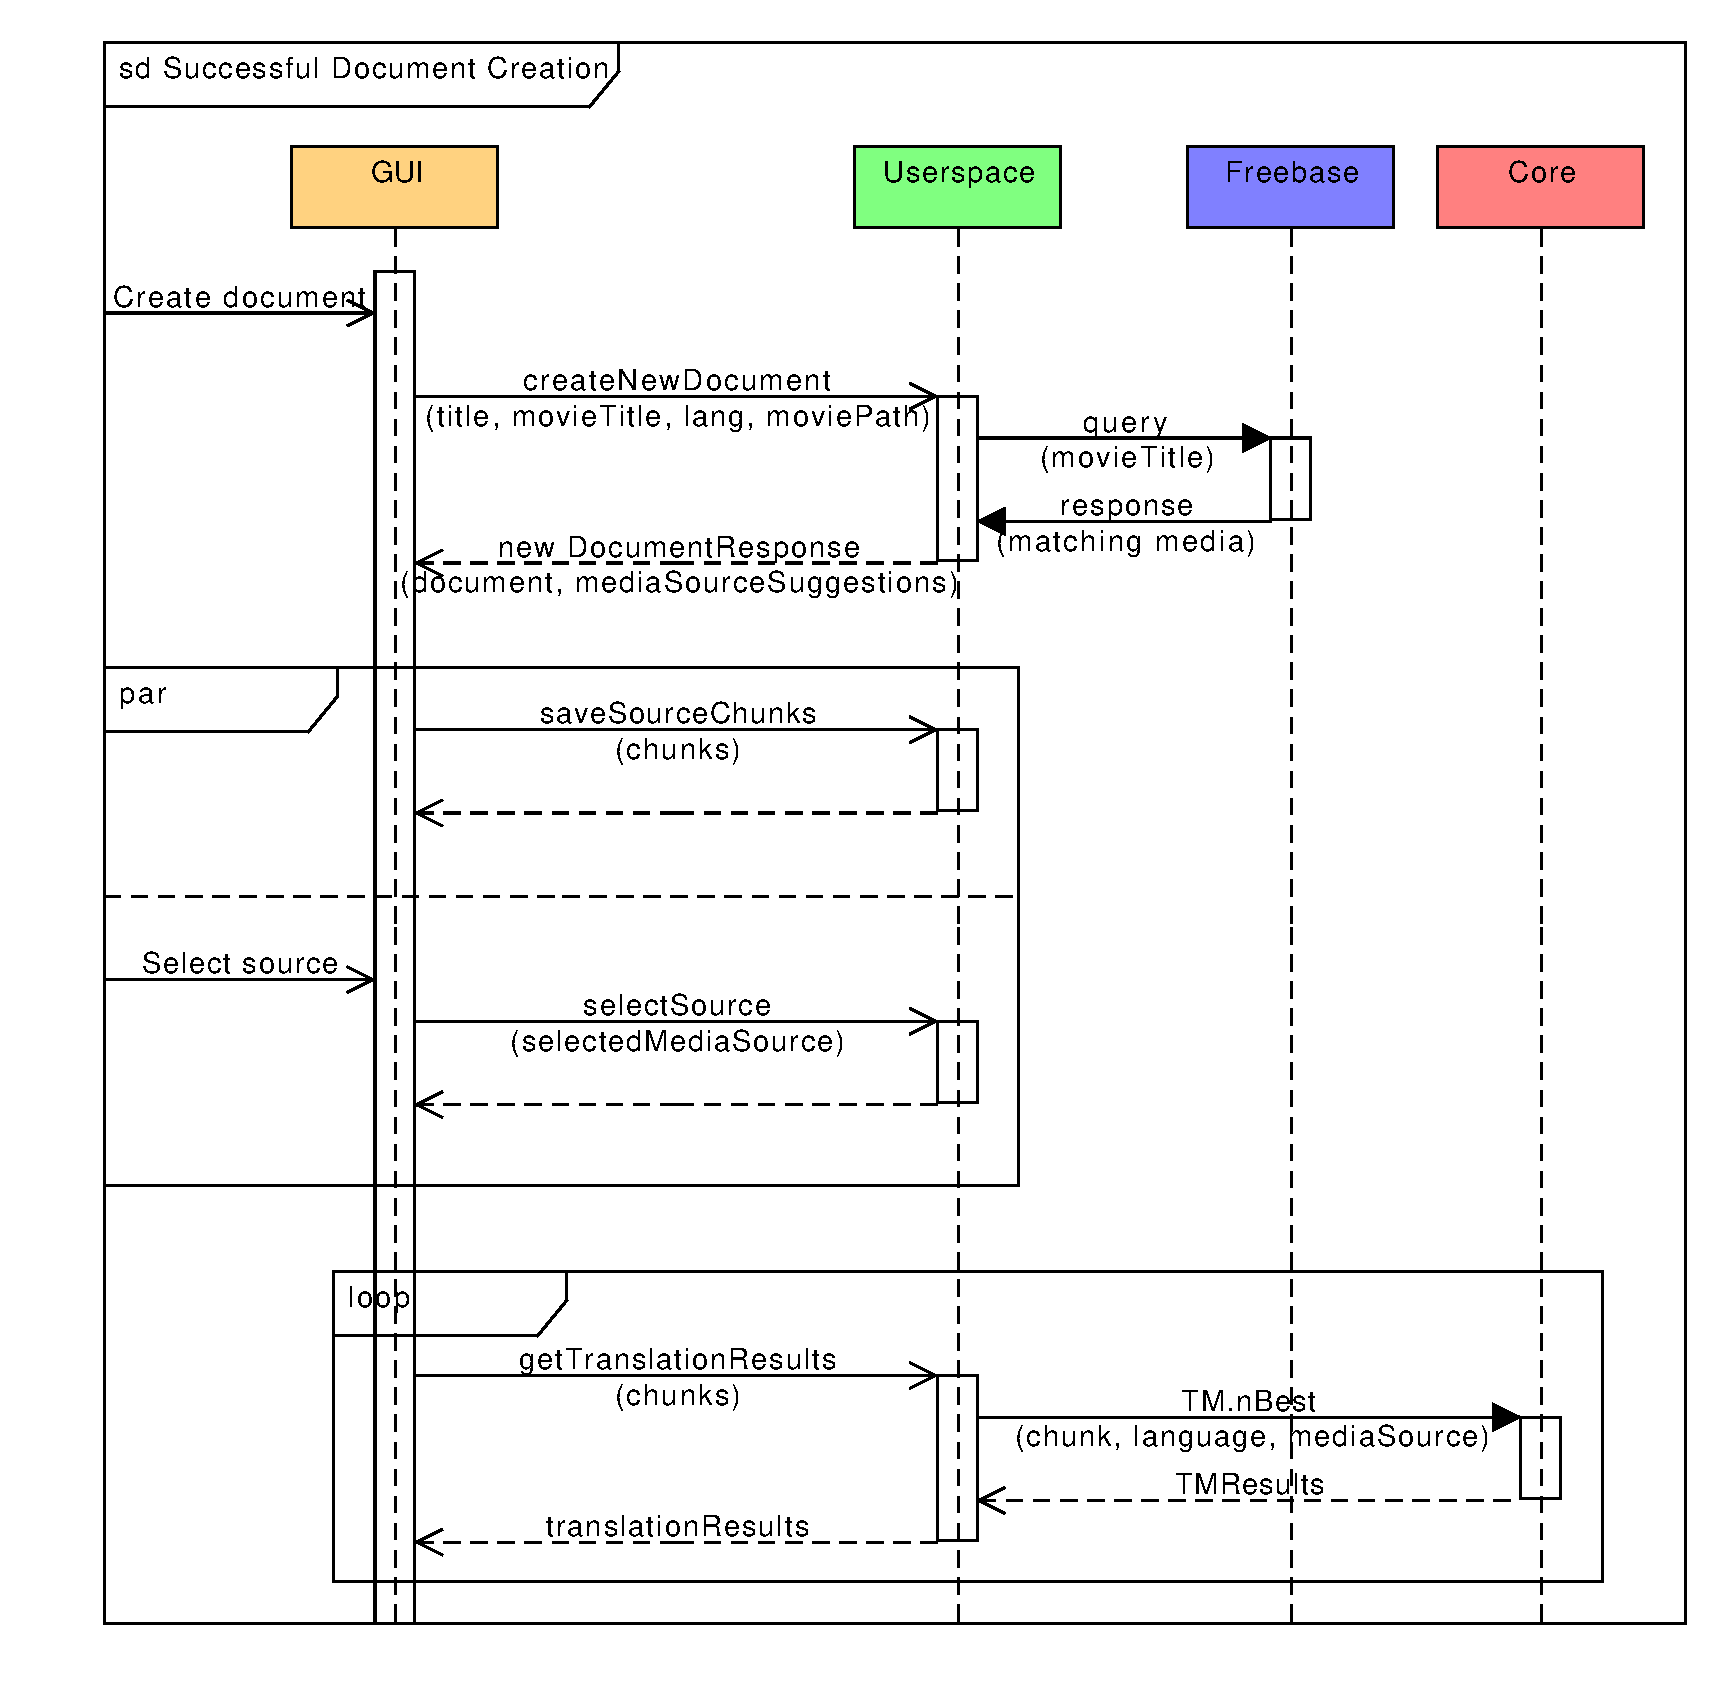
\includegraphics[scale=0.65]{figures/document_creation_sequence_RPC.pdf}
\end{center}
\caption{Sequence diagram of document creation, including translation suggestions loading.}\label{rpc:sd:document_creation}
\end{figure}

\section{User Registration and Login}
\label{sec:rpc:login}

The user is required to log in to use the application.

The users are logged in if they have a valid {\tt sessionID} which is linked to their user accounts.
The {\tt sessionID} expires after a given period of time without any user interaction with the server (1 hour by default).

Two ways to log in are supported -- Simple Login and OpenID Login; these are further described separately. The only two common methods are {\tt checkSessionID} and {\tt logout}, which are therefore described first.

\subsubsection{SessionResponse checkSessionID(String sessionID)}
Validates the given {\tt sessionID}. To be used with a {\tt sessionID} that does not result from invoking neither {\tt simpleLogin} nor {\tt getSessionID} (such as a {\tt sessionID} stored in a cookie).
Returns a {\tt SessionResponse} instance containing the {\tt sessionID} and the {\tt User} object if the {\tt sessionID} is valid, or null otherwise.

\subsubsection{Void logout(String sessionID)}
Invalidate the user session with the given {\tt sessionID}.

\subsection{Simple Login and Registration}
\label{subsec:simple_login}

The Simple Login is the classical implementation of user login. Each user must first register with a unique username and a password of choice. These credentials are then used to log into the application. (The password is to be stored on the server side in the form of a one-way hash.)

The users can also provide an e-mail address for forgotten password retrieval. They then has the option to request a password reset e-mail, based on his username or the e-mail address. The password reset e-mail contains a link to a page where the user can set a new password, based on a temporary password change token.

\subsubsection{Boolean registration(String username, String password, String email)}
Register a user with the given username and password, also setting the e-mail address if provided and sending registration info to it.
Returns true on success, false if the username is already taken, and an exception in case of other errors (usually an invalid e-mail address).

\subsubsection{SessionResponse simpleLogin(String username, String password)}
Try to log in the user with the given username and password.
Returns a {\tt SessionResponse} instance containing the {\tt sessionID} and the User object on success, or null if the credentials are invalid.

\subsubsection{Boolean sendChangePasswordMail(String username)}
Send a password reset e-mail
to the e-mail address of the user with the given username.
Returns true if the e-mail is successfully sent;
returns false if the username is not registered or there is no e-mail address stored with the corresponding user account.

\subsubsection{Boolean sendChangePasswordMailByMail(String email)}
Send a password reset e-mail to the given e-mail address.
The password reset link is bound to a username;
therefore, if there are multiple user accounts with the given e-mail address,
multiple password reset e-mail are sent to the e-mail address.
Returns true if the e-mail is successfully sent;
returns false if the e-mail address is not registered with any user account.

\subsubsection{Boolean changePassword(String username, String password, String token)}
\label{sec:rpc_changePassword}
Set a new password in case of forgotten password.
The temporary password change token must be still valid,
and identical to one sent in the password reset e-mail
to the user with the given username.
Returns true if the password change is successful;
returns false if the token is not valid.

\subsection{Login via OpenID Services}
\label{subsubsec:gui_openid}

This section describes the OpenID Login process. First, the three RPCs involved are introduced. Then, the whole process, also shown in the sequence diagram \ref{rpc:sd:openid_login}, is described.

\subsubsection{LoginSessionResponse getAuthenticationURL(AuthenticationServiceType serviceType)}
\label{sec:rpc_getAuthenticationURL}

Return the URL of a window to show to the user to log in using his OpenID account at an OpenID provider specified by {\tt serviceType}. It leads to a web page of the OpenID provider, with the return page set to the FilmTit application, to the {\tt AuthenticationValidationWindow} page.

A generated temporary one-time identifier, {\tt authID}, is also included in the response. It is used to pair the authentication process, which takes place in the newly opened window, with the main GUI window.

\subsubsection{Boolean validateAuthentication(int authID, String responseURL)}

Validate the response URL from the OpenID provider, which contains information about the result of the OpenID authentication.

If the authentication is found to have been successful, a new session is generated for the user and paired with the given {\tt authID}, and true is returned.
Otherwise, the method returns false.

\subsubsection{SessionResponse getSessionID(int authID)}

Check whether the user has already successfully logged in using his OpenID with the given {\tt authID}.

\begin{itemize}
\item If yes, the corresponding {\tt sessionID} and {\tt User} object are returned.
\item If not yet, but the {\tt authID} is valid, which means that an OpenID login operation is probably still in progress, null is returned.
\item Otherwise, an exception is thrown.
\end{itemize}

\subsubsection{The OpenID login process}
\label{subsubsec:gui:openid}

\begin{figure}[h]
\begin{center}
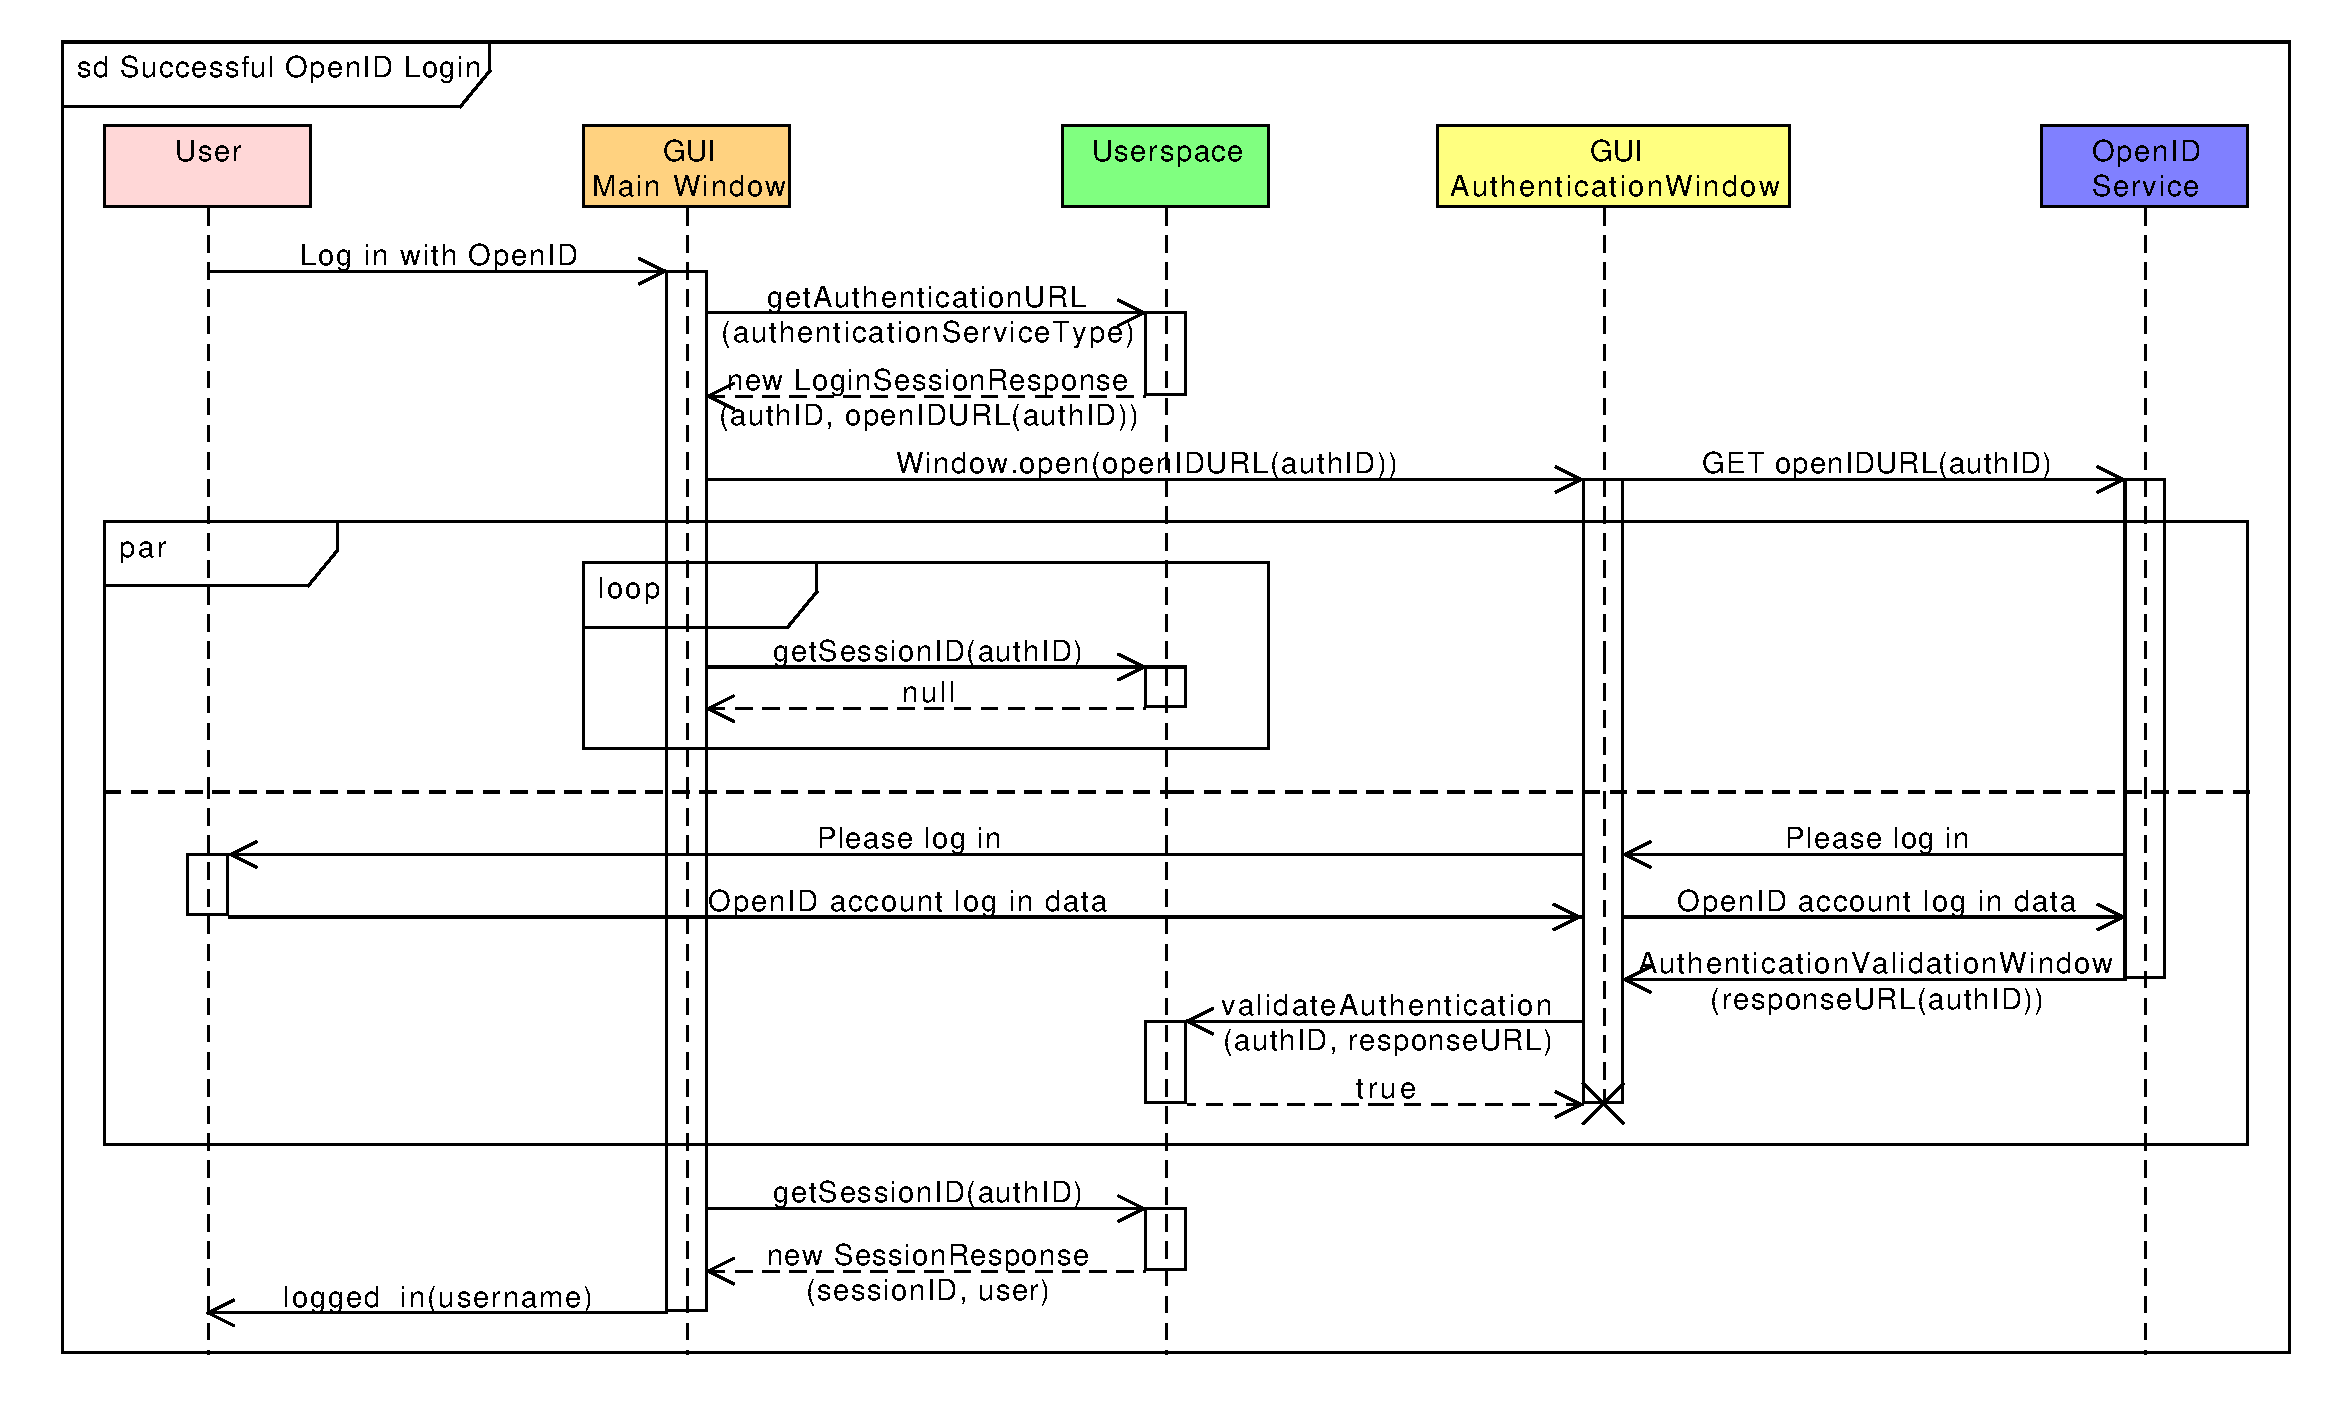
\includegraphics[scale=0.55, angle=90]{figures/openid_login_sequence.pdf}
\end{center}
\caption{Sequence diagram of OpenID login.}\label{rpc:sd:openid_login}
\end{figure}

The authentication itself is done in a new authentication window.
A successful authentication in the authentication window is then paired with the GUI main window using a temporary one-time identifier, {\tt authID}, shared by the User Space, the main GUI window and the authentication window.
(Because of JavaScript security restrictions, there is no simple way of sending the result of the authentication process from the authentication window to the main window;
however, the {\tt authID} can be sent to the new window easily because it is already known at the time of its creation.)

When OpenID Login is requested by the user, the GUI main window calls {\tt getAuthenticationURL} method.
The User Space generates an {\tt authID}, and a URL to be used for the authentication, and returns that to the GUI, which opens a new authentication window with the received URL.
The URL points to an OpenID provider web page (currently supported OpenID providers are Google, Yahoo and Seznam). As a GET parameter, it contains the return URL, which leads back to FilmTit -- to the {\tt AuthenticationValidationWindow} page, including the {\tt authID} as a GET parameter in the return URL.

After opening the authentication window, GUI starts waiting for the user to authenticate. The waiting is active, polling the User Space with {\tt getSessionID} in regular intervals until a non-null value is returned.

Meanwhile, the user can authenticate in the authentication window. The OpenID provider then redirects the user to the return URL, which is the {\tt AuthenticationValidationWindow}, together with parameters describing the result of the authentication and providing some information about the user.
The whole response URL is then sent through {\tt validateAuthentication} to User Space for validation.

If User Space finds the authentication to be successful, a new session is created for the user, and the {\tt sessionID} is stored in a pair with the {\tt authID}.
If a user with the given OpenID is not registered yet, registration is transparently performed at this moment; no explicit registration is required for OpenID login.
The authentication window is then closed.
In case of an error, the error message is displayed in the authentication window (and the window stays open).

When a successful authentication took place, the {\tt getSessionID} method returns the {\tt sessionID} and a {\tt User} object, the polling stops and the authentication process is completed.

\section{User Settings}
\label{sec:rpc:settings}

There are several settings that the user can change. There is a separate call for each of the settings -- therefore, a set of individual calls must be invoked if the user decides to change multiple settings at once, and each of the calls can succeed or fail independently on the results of the other calls.

The settings are stored in the {\tt User} object and sent to GUI on login, as a part of the {\tt SessionResponse} which is the result of the methods {\tt simpleLogin}, {\tt getSessionID} and {\tt checkSessionID}. There is no dedicated method to load the settings; {\tt checkSessionID} is to be used for that purpose.

\subsection{Account and Logging in Settings}

\subsubsection{Void setUsername(String sessionID, String username)}
Change user's username.

\subsubsection{Void setPassword(String sessionID, String password)}
Change user's password.

\subsubsection{Void setEmail(String sessionID, String email)}
Change user's e-mail.

\subsubsection{Void setPermanentlyLoggedIn(String sessionID, boolean permanentlyLoggedIn)}
Stay logged in permanently (for 1 month) instead of 1 hour (sets the session timeout). The time out times configurable, for details see \ref{subsec:user_scpace_settings}.

\subsection{Translation Workspace Settings}

\subsubsection{Void setMaximumNumberOfSuggestions(String sessionID, int number)}
Set maximum number of suggestions to show for each line.

\subsubsection{Void setUseMoses(String sessionID, boolean useMoses)}
Include Machine Translation results in translation suggestions.

\section{Remote Logging}
\label{sec:rpc:remotelog}

The remote logging is used to log messages from GUI on server. The messages are to be printed in the server log and can also be stored in the database.

\subsubsection{Void logGuiMessage(LevelLogEnum level, String context, String message, String sessionID)}
Log the given message from GUI on server.
The supported levels are \emph{DebugNotice}, \emph{Notice}, \emph{Warning} and \emph{Error}.
The context specifies the type of the message and should be constant for each instance of a similar message; it can contain e.g.\ a class name, a method name or an RPC name. The message should be as detailed as to provide all necessary information, including e.g.\ values of variables or a stack trace if applicable.

The {\tt sessionID} is only used to include the {\tt userID} in the logged message; it is to be null if the user is not logged in.

\section{Exceptions Thrown by RPCs}
\label{sec:rpc:exceptions}

The RPCs typically throw an exception on failure. These exceptions should be of only four types, described in this section.

\subsection{InvalidSessionIdException}

Most of the RPCs can only be invoked by a logged in user -- such RPCs take the {\tt sessionID} as their first parameter and throw an {\tt InvalidSessionIdException} in case of an invalid {\tt sessionID}. Typically the ID would be originally valid but expired, so the expected reaction to this exception is to simply ask the user to log in again.

\subsection{InvalidDocumentIdException}

RPCs that manipulate the document usually take the {\tt documentID} as a parameter and throw an {\tt InvalidDocumentIdException} if a document with the given ID does not exist or does not belong to the user.

\subsection{InvalidChunkIdException}

RPCs that manipulate individual chunks take either the whole chunks or only their indexes as a parameter. They throw an {\tt InvalidChunkIdException} if the specified chunk does not exist.

\subsection{InvalidValueException}

The {\tt InvalidValueException} is thrown by a method if a value provided by the user, such as an e-mail address or a password, does not have the required format. It always contains details about the nature of the error as the message, which usually should be shown to the user.


\section{Chunk and Annotations}

Annotations (explained in the Glossary, chapter~\ref{sec:glossary}) were 
initially created for Named Entity Searcher, which marks Named Entities such as Person, Place, Organization (described in greater level in chapter~\ref{core:nent}).

Later, we found out that the same classes can be elegantly used for other features of chunk, like dashes or newlines -- because they are irrelevant for translation (core disregards annotations), but needed for rendering.

Another possible annotation usage for the future is subtitle formatting (bold, italic and underlined text).
However, it seemed to be too complex, especially in the GUI, so we decided to not implement it in the current version of the application, because it is used very little and has no formal specification.

A Chunk has a set of methods to retrieve and set the annotations correctly, using the notion of forms. The forms used are:

\begin{itemize}
	\item \emph{database form:} the text as stored in the subtitle file, only cleaned -- formatting stripped off (bold, italic etc.), non-printable characters turned into spaces, multiple spaces replaced by one space only and newlines are stored as PIPE characters.
	\item \emph{surface form and annotations:} the surface form is the text to be used to generate the translation suggestions, without dashes and with newline turned into spaces
	\item \emph{GUI form:} the HTML form to be displayed in the GUI. Newlines are turned into {\tt <br />} tags.
	\item \emph{text form:} the form to be used in HTML textareas -- with dashes, newlines are generated as {\tt \verb#\n#} characters.
\end{itemize}
